%----------------------------------------------------------------------------------------
%	PACKAGES AND THEMES
%----------------------------------------------------------------------------------------

\documentclass{beamer}

\mode<presentation> {

\usetheme{Singapore}
\usecolortheme{seahorse}

%\setbeamertemplate{footline} % To remove the footer line in all slides uncomment this line
%\setbeamertemplate{footline}[page number] % To replace the footer line in all slides with a simple slide count uncomment this line
%\setbeamertemplate{navigation symbols}{} % To remove the navigation symbols from the bottom of all slides uncomment this line
}

%%%% HELPFUL REFERENCE FOR THE PRESENTATION
% https://ryanstutorials.net/bash-scripting-tutorial/

\usepackage{amsmath}
\usepackage{graphicx} % Allows including images
\usepackage{booktabs} % Allows the use of \toprule, \midrule and \bottomrule in tables

% CAPTIONS
\usepackage{subfig}

%\usepackage{sectsty} % Allows customizing section commands
%\allsectionsfont{\centering \normalfont\scshape} % Make all sections centered, the default font and small caps

\newcommand{\mb}{\mathbf}
\newcommand{\tb}{\textbf}
\newcommand{\ti}{\textit}
\newcommand{\ul}{\underline}
\newcommand{\bi}{\begin{itemize}}
\newcommand{\ei}{\end{itemize}}
\newcommand{\be}{\begin{enumerate}}
\newcommand{\ee}{\end{enumerate}}

% Non-shown text to appear gray
\setbeamercovered{transparent}

% NO HYPHENATION TEST
\usepackage[none]{hyphenat}

% FANCY FOOTNOTE SYMBOLS
\renewcommand*{\thefootnote}{\fnsymbol{footnote}}

\renewcommand{\baselinestretch}{1.2}

%%%%%%%%%%%%%%%%%%%%%%%%%%%%%%%%%%%%%%%%%%%%%%%%



\title[Server]{Bash Scripts \& Acropolis: Using the SSCS Servers}
\institute{\large{EPIC RA Orientation}}
\date{August 20, 2018}

\logo{
\centering

\includegraphics[scale=0.2]{epic_logo}
}



%%%%%%%%%%%%%%%%%%%%%%%%%%%%%%%%%%%%%%%%%%%%%%%%%%%%%%%%%%%%%%%%%%%%%
\begin{document}

\begin{frame}
	\titlepage
\end{frame}

\section{Command Line}
\begin{frame}
	\frametitle{What is the Command Line?}
	Method of interacting with computer program (in our case, file structure) using successive lines of text within the terminal (Mac, Linux) or terminal emulator (Windows). 
	\\[1em]\pause
	In Mac, go to Launchpad $\to$ Search Bar $\to$ Terminal.
	\\
	In Windows, open PuTTY or equivalent. 
	\\[1em]
	\tiny{It has been 3 years since I've used any terminal emulator on Windows, so the presentation will focus on using Terminal in Mac.}
	\\[1em]
	\tiny{NOTE: All commands in this presentation are shown using the \textsc{textsc} font. When entering commands in the command line, use all lower case unless otherwise noted}s
\end{frame}


\begin{frame}
	\frametitle{Commonly used Command Line commands}
	\bi
		\item \textsc{cd} [dir]: change directory to [dir]
		\bi	
			\item relative vs absolute paths, .. to move up a folder
		\ei
		\item \textsc{ls}: list files
		\item \textsc{mv} [a] [b]: move or rename file [a] to [b]
		\item \textsc{man} [cmd]: manual for command [cmd] with all the flags
		\item \textsc{mkdir} [dir]: creates a new directory [dir]
		\item \textsc{touch} [fname]: creates a new empty file [fname]
	\ei
	Don't delete files using rm unless you are very comfortable. Permanent deletion.
\end{frame}

\begin{frame}
	\frametitle{Other useful Command Line commands}
	\bi
		\item \textsc{cat} [file]: Prints the content of the file [file].
		\item \textsc{head} -n [$X$] [file]: First [$X$] lines of the file [file]
		\item \textsc{tail} -n [$X$] [file]: Last [$X$] lines of the file [file]
		\item \textsc{grep} [str] [files]: Searching plain-text files (e.g. logs) for the regular expression [str] in the files [files]
		\item Ctrl + C: Force quit
	\ei
\end{frame}

\begin{frame}
	\frametitle{Command Line Stata}
	It is possible to run Stata from the command line. Just type \textsc{stata} in Terminal.
	\\[1em]\pause
	However, for better control, run Stata via scripts. This is our preferred method for submitting Stata tasks to the server.
\end{frame}

\section{Scripts}
\begin{frame}
	\frametitle{What is a script?}
	A set of Command Line commands, along with the conditions on which they are run.
	\\[1em]
	\pause
	Bash is a command processor that can read and execute commands from a shell script. Think of Bash as an implementation of a shell and think of a shell as the user interface to the operating system.
\end{frame}

\begin{frame}
	\frametitle{Components of a Bash script}
	\begin{figure}
		\centering
		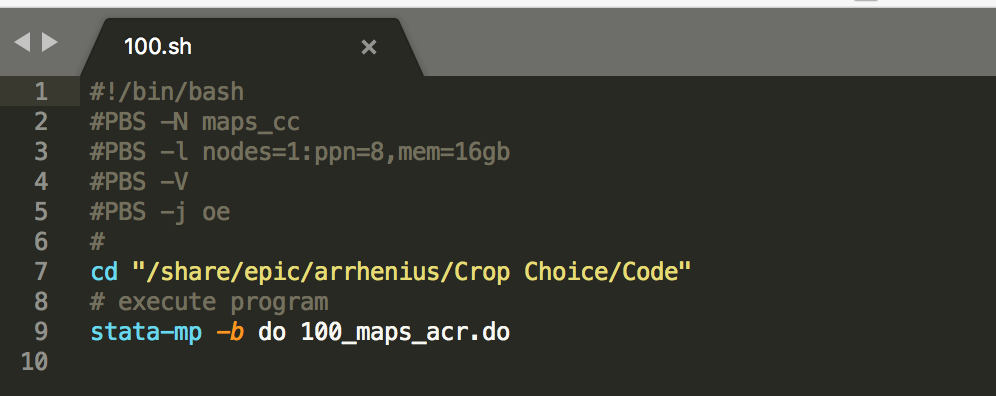
\includegraphics[width=0.8\linewidth]{bash}
	\end{figure}
	\pause
	\small{Line 1: Must be ``\#!/bin/bash'', the path to the (bash) interpreter to run the program
	\\[0.5em]
	Lines 2-5: Portable Batch System (PBS) environment conditions for running the script. -N is the name. -l specifies the computing resources. }
\end{frame}

\section{Acropolis}
\begin{frame}
	\frametitle{What is Acropolis}
	Acropolis is the economics computing cluster, overseen by the Social Sciences Computing Services (SSCS).
\end{frame}

\begin{frame}
	\frametitle{How do I access Acropolis?}
	\small{One way is via the command line using secure shell (ssh):}
	\begin{figure}
		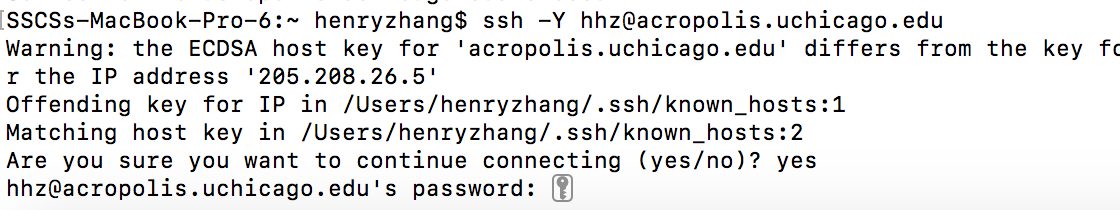
\includegraphics[width=0.6\linewidth]{ssh}
	\end{figure}
	\small{After logging in,}
	\begin{figure}
		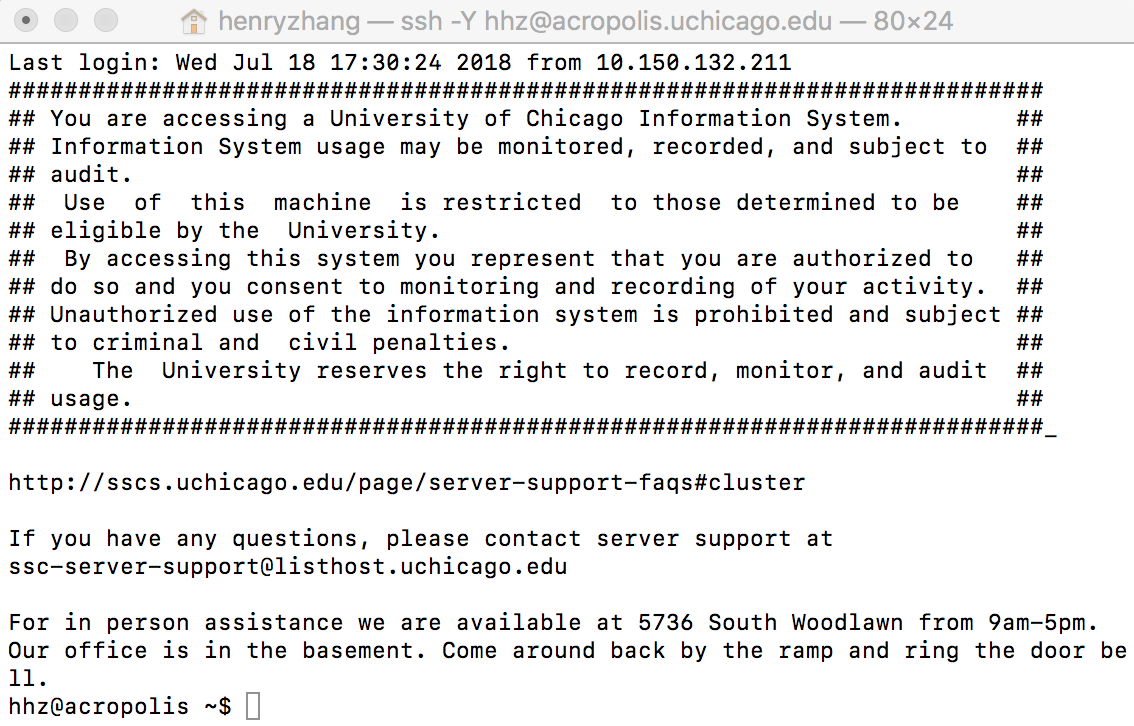
\includegraphics[width=0.6\linewidth]{ssh_acropolis}
	\end{figure}
\end{frame}

\begin{frame}
	\frametitle{How do I access Acropolis?}
	Another way is via a GUI like Cyberduck. Cyberduck allows you to quickly download/upload and directly edit files on Acropolis, but is prone to crashing.
	\begin{figure}
		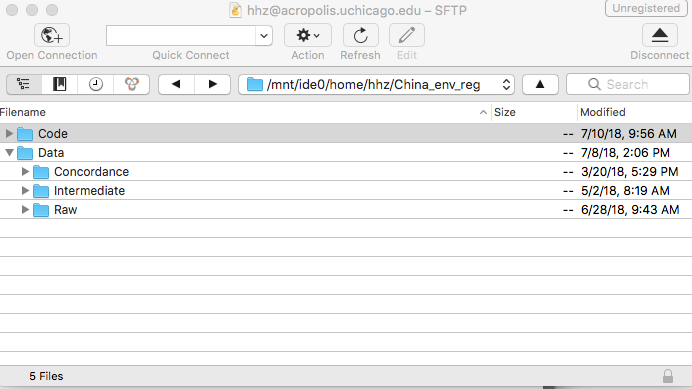
\includegraphics[width=0.6\linewidth]{cyberduck}
	\end{figure}	
\end{frame}


\begin{frame}
	\frametitle{Acropolis tips: Running a script}
	Use \textsc{cd} to go the directory of the script file. 
	\\
	Type \textsc{nohup qsub} [scriptname] \&
	\bi
		\item \textsc{nohup}: Command to ignore the hangup signal (hup). Allows commands to continue running undisturbed when you log out of your Acropolis session
		\item \textsc{qsub}: Submit an executable script to the batch server
		\item \& returns control of the command line to the user (otherwise, you would not have control until the script is done)
	\ei
	This will automatically create a log file for each do-file you run. 
	% Batch job is program assigned to computer without further user interaction
\end{frame}

\begin{frame}
	\frametitle{Checking a script}
	Type \textsc{qstat} to see the status of all your scripts, by the name you listed in -N
	\\[1em]
	\pause
	If you want to delete a script, type \textsc{qdel} and then the name of the script that appears from \textsc{qstat}, e.g. ``137342.acropolis''
\end{frame}

\begin{frame}
	\frametitle{Acropolis tips}
	\bi[<+>]
		\item Apply for an account at ``https://iota.src.uchicago.edu/''. Just mention whom you work for and what you'll do with your server access
		\item Your root directory is ``/home/[your username]''
		\item Use \textsc{tail} -n 10 [log file name] to quickly see if any issues arose (specifically in Stata, error codes)
		\item Be conscientious about how much memory you allocate. You likely do not need more than 16GB. Most tasks are CPU-constrained, not memory-constrained.
		% Contact Steve Mohr at SSCS if you have any Acropolis questions that other RAs can't figure out
	\ei
\end{frame}

\begin{frame}
	\frametitle{Stata on Acropolis tips}
	\bi[<+>]
		\item If you receive a message like ``unable to write to [...] file'', the likely culprit is a nonexistent or misspecified Acropolis directory
		\item Do \textbf{not} include any pause statements in any do-file you run on the server. This will cause the program to incessantly cycle and the log file will balloon due to the repeated error message that pausing is not allowed. 
		\item If you have a file that you plan to run interactively (for debugging) and also on the server, create a local switch `acropolis' at the top of your do-file and if `acropolis' == 1, then set pause off
	\ei
\end{frame}

\end{document}
